\chapter{Sistemas Numéricos, Memória e Compilação}
\label{cap:sistemas-numericos}

Antes de avançar pela sintaxe da linguagem, vale entender melhor o terreno sobre o qual ela é construída: como um computador representa números, como organiza a memória e o que, de fato, acontece entre escrever um arquivo \code{.c} e obter um programa executável. Esses fundamentos são especialmente relevantes em sistemas embarcados, onde memória é escassa e o programador frequentemente manipula dados diretamente em binário e hexadecimal.

\section{Sistema binário}

Computadores armazenam e processam informação usando apenas dois estados elétricos — ligado e desligado —, representados matematicamente pelos dígitos \(0\) e \(1\). Esse é o \textbf{sistema binário} (base 2). Cada dígito binário é chamado de \textbf{bit} (\emph{binary digit}); um grupo de 8 bits forma um \textbf{byte}.

Um número binário é interpretado da mesma forma que um número decimal, mas com potências de 2 em vez de potências de 10:

\[
1011_2 = 1\times2^3 + 0\times2^2 + 1\times2^1 + 1\times2^0 = 8+0+2+1 = 11_{10}
\]

\begin{table}[h]
\centering
\begin{tabular}{@{}cccc@{}}
\toprule
\textbf{Bits} & \textbf{Nome} & \textbf{Valores possíveis} & \textbf{Intervalo (sem sinal)} \\
\midrule
1 & bit      & 2         & 0 a 1 \\
4 & nibble   & 16        & 0 a 15 \\
8 & byte     & 256       & 0 a 255 \\
16 & word (na maioria dos MCUs de 16b) & 65\,536 & 0 a 65\,535 \\
32 & double word & 4\,294\,967\,296 & 0 a $2^{32}-1$ \\
\bottomrule
\end{tabular}
\caption{Grupos comuns de bits e sua capacidade de representação.}
\end{table}

\section{Sistemas octal e hexadecimal}

Escrever endereços de memória ou máscaras de bits inteiramente em binário é verboso e propenso a erros. Por isso, é comum usar bases que sejam potências de 2 e que reduzam o número de dígitos: o \textbf{octal} (base 8) e, principalmente, o \textbf{hexadecimal} (base 16).

No hexadecimal, os dígitos vão de 0 a 9 e depois de A a F (representando 10 a 15). Cada dígito hexadecimal representa exatamente 4 bits (um nibble), o que torna a conversão entre binário e hexadecimal praticamente mecânica:

\begin{table}[h]
\centering
\begin{tabular}{@{}cccc@{}}
\toprule
\textbf{Decimal} & \textbf{Binário} & \textbf{Octal} & \textbf{Hexadecimal} \\
\midrule
0  & 0000 & 0  & 0 \\
7  & 0111 & 7  & 7 \\
10 & 1010 & 12 & A \\
15 & 1111 & 17 & F \\
255 & 1111 1111 & 377 & FF \\
\bottomrule
\end{tabular}
\caption{Um mesmo valor em diferentes bases numéricas.}
\end{table}

Em C, cada base tem uma notação própria para constantes literais:

\begin{codigoc}{Notação de bases numéricas em C}
int decimal     = 42;        // Base 10 (padrao)
int octal       = 052;       // Base 8  (prefixo 0)
int hexadecimal = 0x2A;      // Base 16 (prefixo 0x)
int binario     = 0b101010;  // Base 2  (prefixo 0b, extensao GNU/C23)
\end{codigoc}

\begin{atencao}
O prefixo \code{0} para octal é uma pegadinha clássica: escrever \code{int codigo = 057;} pensando em ``cinquenta e sete'' na verdade produz o valor 47 em decimal, porque o compilador interpreta o zero à esquerda como indicação de base octal.
\end{atencao}

\begin{esp32box}
Hexadecimal é a notação padrão para endereços de memória e para os \textbf{registradores} de periféricos do \ESP{} (ex.: \code{0x3FF44004}), e é extremamente comum representar conjuntos de pinos GPIO como \textbf{máscaras de bits} em binário ou hexadecimal — cada bit ligado corresponde a um pino específico habilitado. Voltaremos a essa ideia no \cref{cap:gpio}, quando configurarmos registradores de GPIO diretamente.
\end{esp32box}

Se você assistiu ao filme \emph{Perdido em Marte} (ou leu o livro de Andy Weir), viu o sistema hexadecimal resolver um problema vital de engenharia. No enredo, o astronauta Mark Watney precisa se comunicar com a Terra usando a câmera giratória da antiga sonda \href{https://science.nasa.gov/mission/mars-pathfinder/}{Mars Pathfinder}.

\begin{figure}[H]
\centering
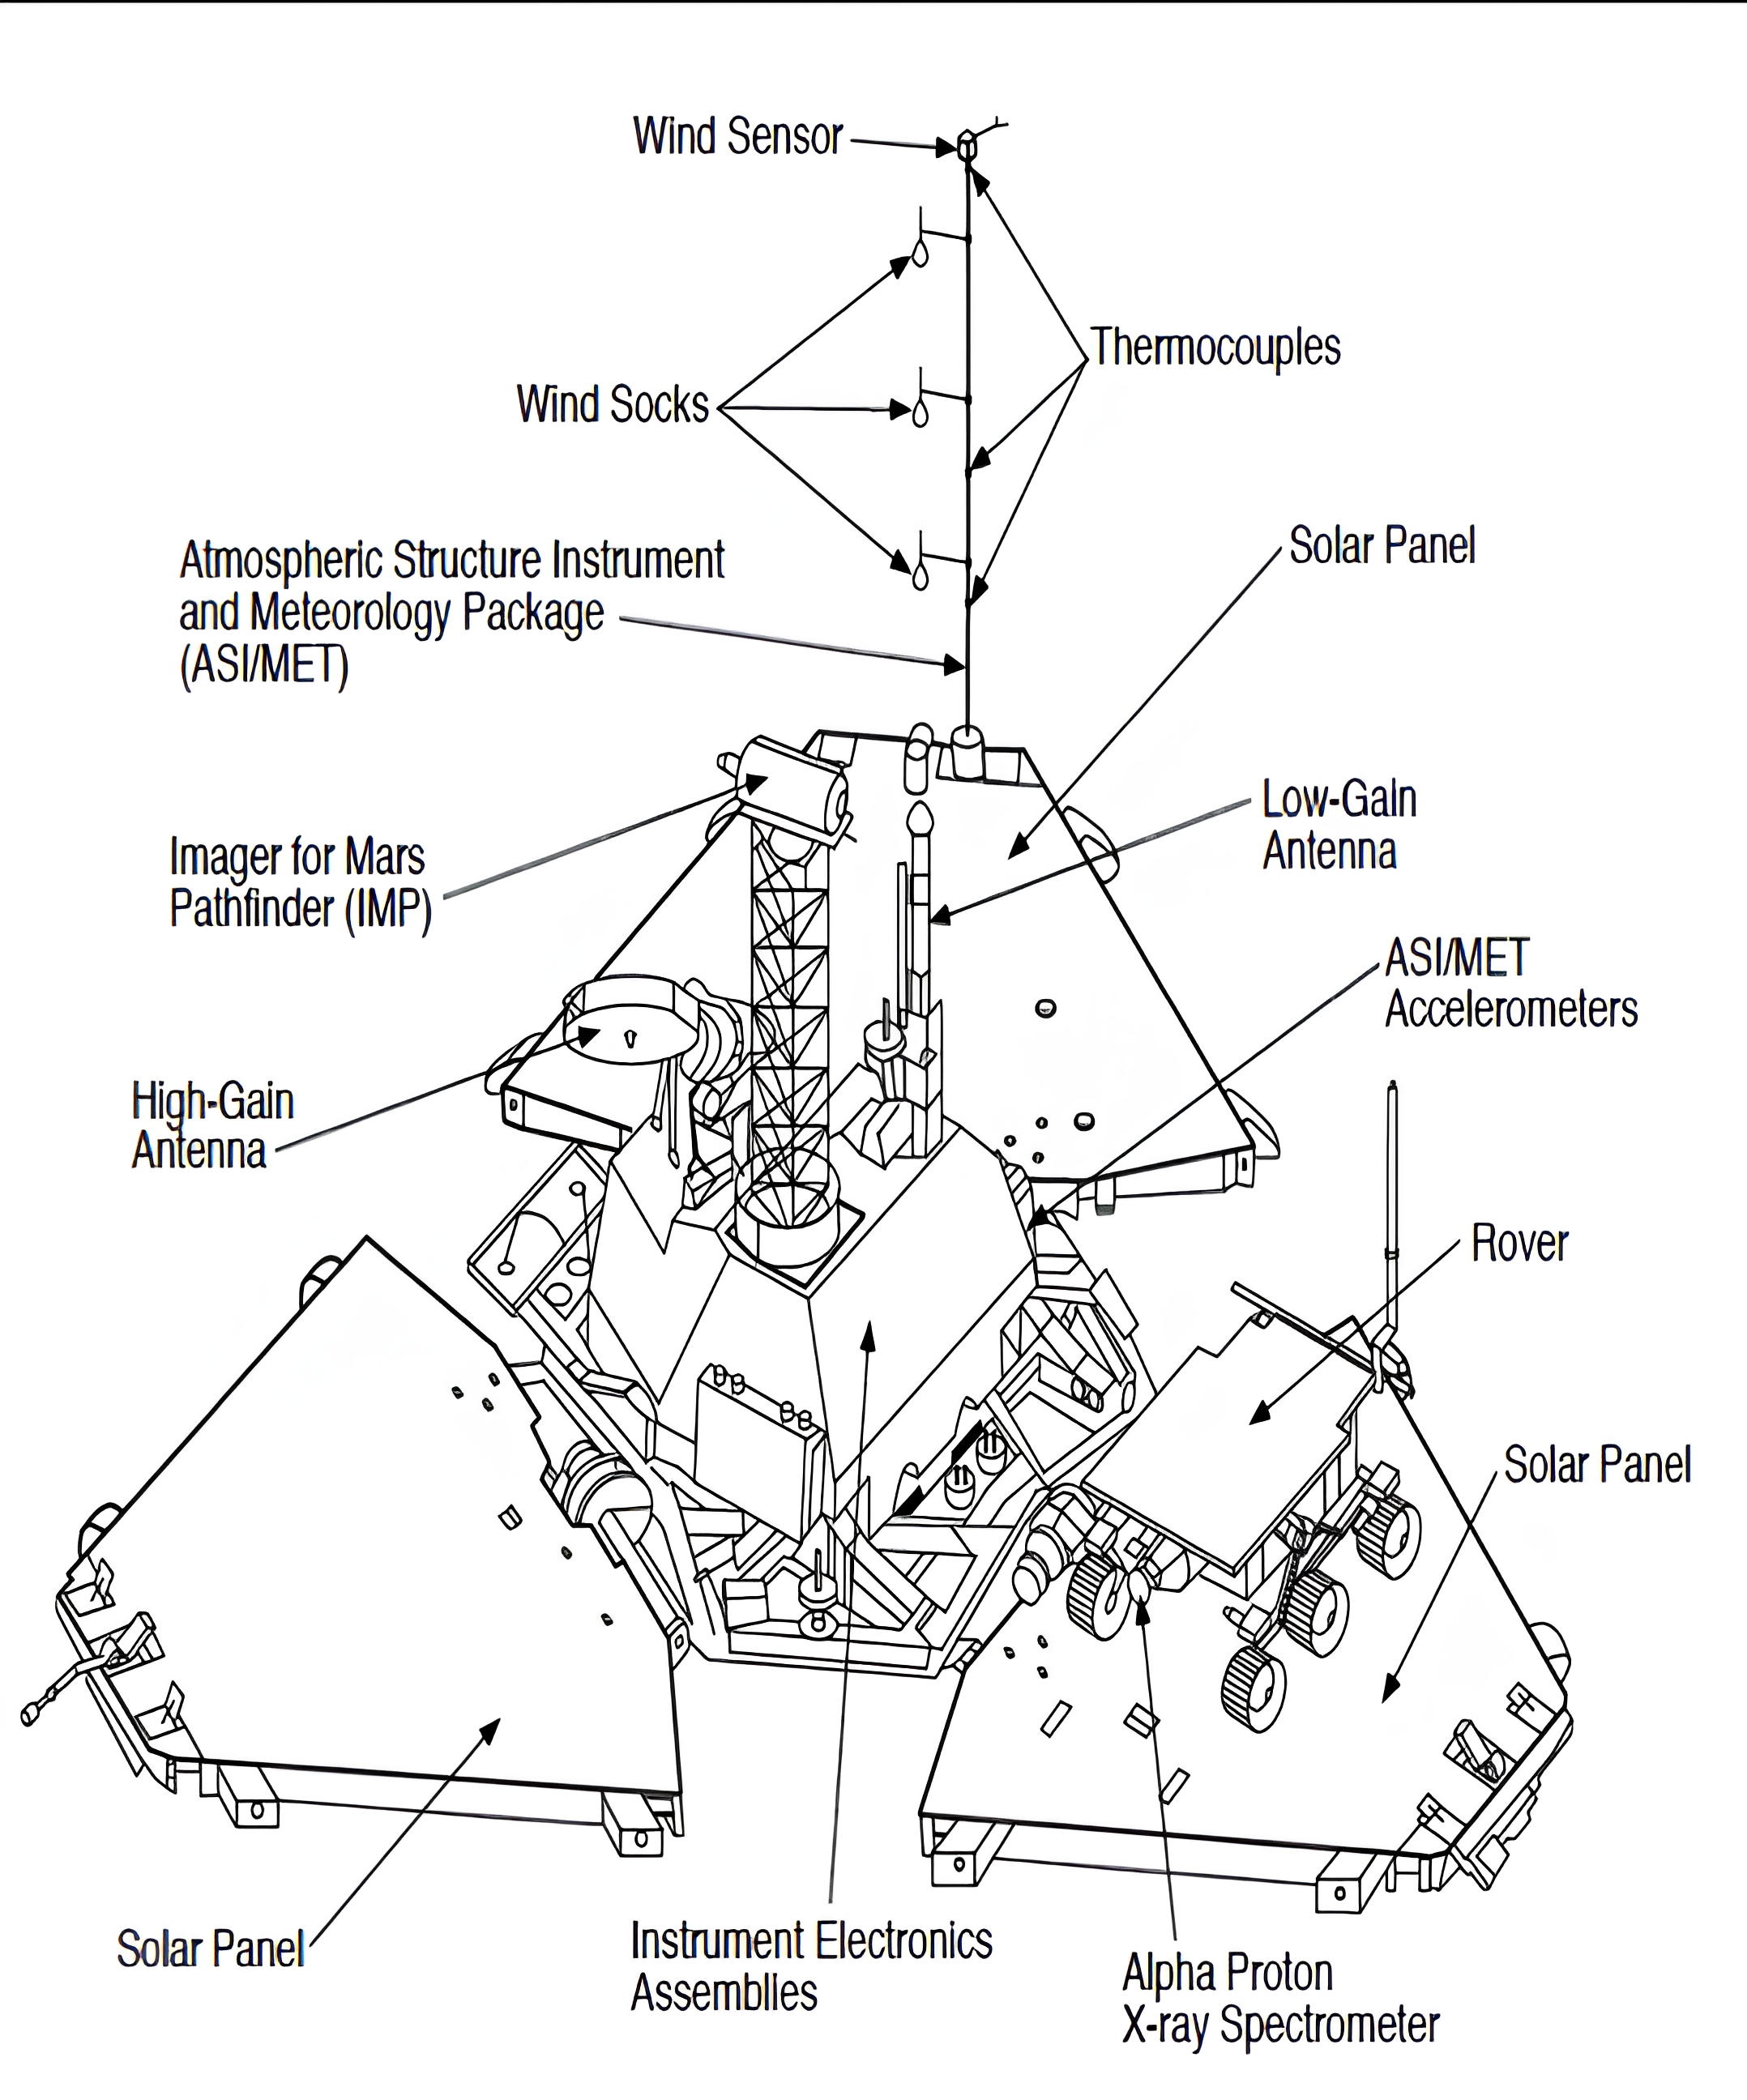
\includegraphics[width=0.7\textwidth]{imagens/mars_pathfinder.png}
\caption{Diagrama da plataforma de pouso da missão Mars Pathfinder da NASA. Repare na câmera rotatória acoplada ao sistema.}
\end{figure}

Ele precisava que a câmera apontasse para placas com letras ao seu redor. Se usasse o alfabeto convencional (26 letras), ele teria que dividir os 360 graus do círculo por 26, o que dá fatias estreitas de cerca de 13,8 graus. A chance de a câmera apontar para a fronteira entre duas letras e gerar ambiguidade era enorme.

A solução? Usar a tabela ASCII (que mapeia texto em números) em formato \textbf{hexadecimal}. Como o hexadecimal possui apenas 16 símbolos (0 a 9 e A a F), ele pôde dividir os 360 graus por 16. O resultado foram fatias largas e seguras de 22,5 graus. Assim, para a Terra enviar a letra "H" (cujo valor na tabela ASCII é 72 em decimal, ou \code{0x48} em hexadecimal), a câmera girava primeiro para a placa \code{4} e depois para a placa \code{8}.

\begin{figure}[H]
\centering
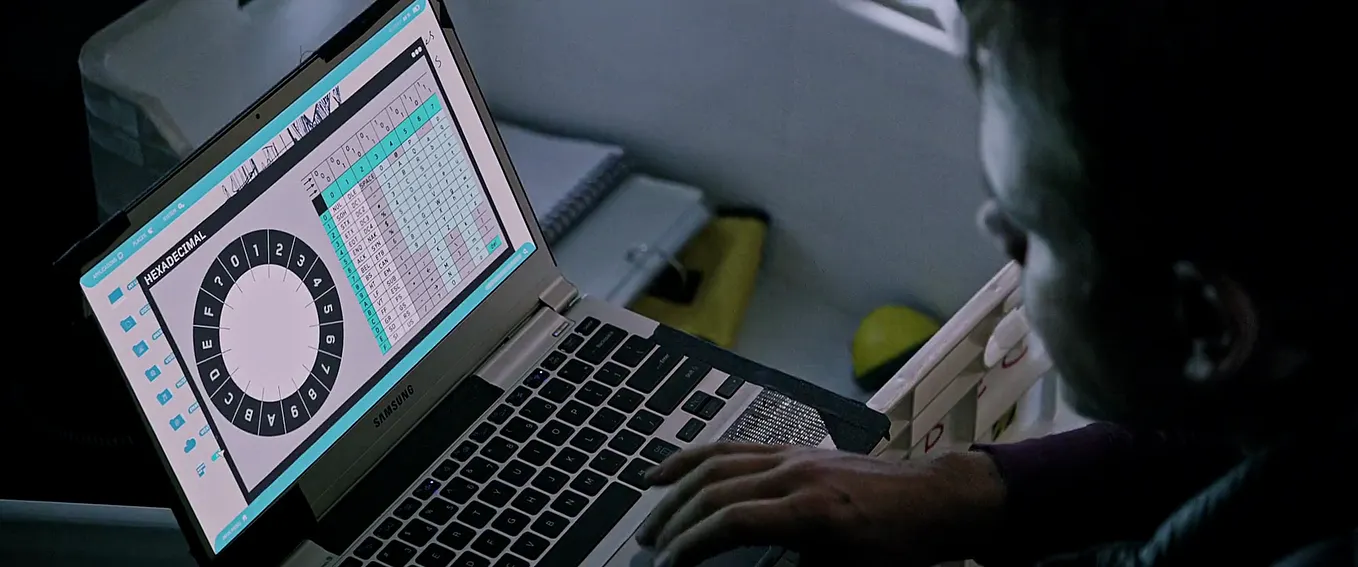
\includegraphics[width=0.8\textwidth]{imagens/mark_watney.png}
\caption{Mark Watney acessando a tabela ASCII pelo notebook de Beth Johanssen.}
\end{figure}

A cena do primeiro contato do filme pode ser vista neste \href{https://www.youtube.com/watch?v=NttUBB98zg4}{link Youtube}.

\section{Memória}

Um programa em execução manipula dados que residem na \textbf{memória} do sistema. Em um computador de propósito geral, essa memória é tipicamente volátil (RAM) e vasta (gigabytes); o sistema operacional gerencia sua alocação de forma praticamente transparente ao programador.

Um microcontrolador como o \ESP{} tem uma realidade bem diferente:

\begin{itemize}
    \item \textbf{Flash} — memória não volátil (mantém os dados sem energia), onde o firmware compilado é gravado. No \ESP{}, tipicamente 4~MB ou mais;
    \item \textbf{SRAM} — memória volátil, rápida, usada para variáveis, pilha (\emph{stack}) e heap durante a execução. No \ESP{}, apenas algumas centenas de kB — ordens de magnitude menor que a RAM de um computador comum.
\end{itemize}

Essa escassez de memória é a razão pela qual, em programação embarcada, escolher o \textbf{tipo de dado} correto para cada variável (assunto do \cref{cap:tipos}) deixa de ser um preciosismo e passa a ser uma decisão de engenharia: usar um \code{int} de 32 bits para armazenar um valor que cabe perfeitamente em 8 bits desperdiça memória que, em um sistema embarcado, pode ser exatamente o que falta.

\section{Pré-processamento}
\label{sec:preprocessamento}

Antes que o compilador propriamente dito veja o código, ele passa por um estágio chamado \textbf{pré-processamento}, controlado por linhas que começam com \code{\#} — as \textbf{diretivas}. Já vimos uma delas, \code{\#include}. Outras diretivas comuns:

\begin{codigoc}{Diretivas de pré-processador}
#include <stdio.h>               // inclui um cabecalho da biblioteca padrao
#include "meu_arquivo.h"         // inclui um cabecalho do proprio projeto

#define PI 3.14159               // define uma macro/constante simbolica
#define QUADRADO(x) ((x) * (x))  // macro com "parametro"

#ifdef DEBUG
    printf("Modo debug ativo\n");
#endif
\end{codigoc}

A diretiva \code{\#define} cria uma \textbf{macro}: onde quer que \code{PI} apareça no código depois dessa linha, o pré-processador o substitui literalmente por \code{3.14159}, \emph{antes} mesmo de o compilador analisar a sintaxe. Diretivas condicionais como \code{\#ifdef}/\code{\#endif} permitem incluir ou excluir trechos inteiros de código dependendo de configurações — um recurso muito usado em projetos embarcados para, por exemplo, ativar mensagens de depuração apenas em builds de desenvolvimento.

Veja como isso se aplica na prática em um código para o ESP32. Podemos criar uma macro chamada \code{DEBUG} e usá-la para "ligar" ou "desligar" o envio de dados pela porta serial:

\begin{codigoc}{Depuração condicional com macros}
#define DEBUG  // Comente esta linha (coloque // na frente) para desativar o debug

void setup() {
    // Inicializa a serial (nao tem problema inicializar mesmo sem usar)
    Serial.begin(115200);

    #ifdef DEBUG
        Serial.println("Sistema iniciado. Modo DEBUG ativo.");
    #endif
}

void loop() {
    int leitura = analogRead(34); // Leitura de um sensor qualquer

    #ifdef DEBUG
        Serial.print("Valor lido pelo sensor: ");
        Serial.println(leitura);
    #endif

    // A logica principal do programa continua aqui, 
    // sem interrupcoes da serial se o DEBUG estiver desativado
    delay(1000);
}
\end{codigoc}

Essa técnica é extremamente poderosa. Ela permite que você encha o seu código de mensagens úteis para investigar o comportamento do sistema durante o desenvolvimento. Quando o projeto estiver pronto para uso real, basta comentar a primeira linha (\code{// \#define DEBUG}). O pré-processador, então, apagará invisivelmente tudo o que estiver entre os blocos \code{\#ifdef DEBUG} e \code{\#endif} antes da compilação. O resultado? Um firmware final menor, mais rápido e que não desperdiça processamento enviando texto para uma porta USB vazia.

\section{Compilação}
\label{sec:compilacao}

O termo ``compilar'' esconde, na verdade, quatro etapas distintas:

\begin{enumerate}
    \item \textbf{Pré-processamento} — expande \code{\#include}, \code{\#define} e diretivas condicionais, produzindo um único arquivo de código-fonte ``puro'';
    \item \textbf{Compilação} — traduz o código C em código assembly equivalente para a arquitetura de destino;
    \item \textbf{Montagem (\emph{assembly})} — converte o código assembly em código de máquina, gerando um arquivo objeto (\code{.o});
    \item \textbf{Ligação (\emph{linking})} — combina o(s) arquivo(s) objeto com as bibliotecas necessárias (como a implementação de \code{printf}) em um único executável.
\end{enumerate}

O \code{gcc} executa essas quatro etapas automaticamente, mas é possível observá-las de forma isolada com a seguir:

\begin{codigobash}{Etapas de compilação separadas}
$ gcc -E hello_world.c -o hello_world.i   # so o pre-processador
$ gcc -S hello_world.i -o hello_world.s   # gera assembly
$ gcc -c hello_world.s -o hello_world.o   # gera arquivo objeto
$ gcc hello_world.o -o hello_world        # linka e gera o executavel
\end{codigobash}

\begin{esp32box}
Ao compilar um projeto para o \ESP{} no PlatformIO, essas mesmas quatro etapas acontecem — só que usando um compilador \textbf{cruzado} (\emph{cross-compiler}): o código roda no seu computador (arquitetura x86/ARM), mas o binário gerado é destinado a um processador \textbf{Xtensa} (a arquitetura do \ESP{}), completamente diferente. O PlatformIO baixa e gerencia essa toolchain de compilação cruzada automaticamente — é uma das razões pelas quais ele simplifica tanto o processo. Detalhes no \cref{cap:platformio}.
\end{esp32box}

\section{Números pseudoaleatórios}

Muitos programas — jogos, simulações, e também firmwares embarcados — precisam de números aparentemente aleatórios. Como um computador é uma máquina determinística, ele não gera aleatoriedade verdadeira a partir do nada: gera números \textbf{pseudoaleatórios}, calculados por uma fórmula a partir de um valor inicial chamado \textbf{semente} (\emph{seed}).

\begin{codigoc}{Gerando números pseudoaleatórios}
#include <stdio.h>
#include <stdlib.h>
#include <time.h>

int main(void) {

    srand(time(NULL));          // inicializa a semente com o tempo atual
    int dado = (rand() % 6) + 1; // numero pseudoaleatorio entre 1 e 6

    printf("Voce tirou: %d\n", dado);
    return 0;
}
\end{codigoc}

A função \code{srand} define a semente do gerador; usar \code{time(NULL)} (o tempo atual em segundos) garante uma semente diferente a cada execução. A função \code{rand()} retorna um valor inteiro pseudoaleatório; o operador \code{\%} (resto da divisão) é usado para restringir o resultado a um intervalo específico — no exemplo, de 1 a 6, como em um dado de tabuleiro.

\begin{atencao}
\code{rand()} \textbf{não} é adequado para fins criptográficos — sua sequência é previsível se a semente for conhecida. Para geração de números aleatórios seguros, bibliotecas específicas de criptografia devem ser usadas.
\end{atencao}
